% Options for packages loaded elsewhere
\PassOptionsToPackage{unicode}{hyperref}
\PassOptionsToPackage{hyphens}{url}
\PassOptionsToPackage{dvipsnames,svgnames,x11names}{xcolor}
\PassOptionsToPackage{space}{xeCJK}
\documentclass[
  11pt,
]{article}
\usepackage{xcolor}
\usepackage[margin=0.9in]{geometry}
\usepackage{amsmath,amssymb}
\setcounter{secnumdepth}{-\maxdimen} % remove section numbering
\usepackage{iftex}
\ifPDFTeX
  \usepackage[T1]{fontenc}
  \usepackage[utf8]{inputenc}
  \usepackage{textcomp} % provide euro and other symbols
\else % if luatex or xetex
  \usepackage{unicode-math} % this also loads fontspec
  \defaultfontfeatures{Scale=MatchLowercase}
  \defaultfontfeatures[\rmfamily]{Ligatures=TeX,Scale=1}
\fi
\usepackage{lmodern}
\ifPDFTeX\else
  % xetex/luatex font selection
  \setmainfont[]{TeX Gyre Termes}
  \setmathfont[]{TeX Gyre Termes Math}
  \ifXeTeX
    \usepackage{xeCJK}
    \setCJKmainfont[]{Noto Serif CJK SC}
  \fi
  \ifLuaTeX
    \usepackage[]{luatexja-fontspec}
    \setmainjfont[]{Noto Serif CJK SC}
  \fi
\fi
% Use upquote if available, for straight quotes in verbatim environments
\IfFileExists{upquote.sty}{\usepackage{upquote}}{}
\IfFileExists{microtype.sty}{% use microtype if available
  \usepackage[]{microtype}
  \UseMicrotypeSet[protrusion]{basicmath} % disable protrusion for tt fonts
}{}
\makeatletter
\@ifundefined{KOMAClassName}{% if non-KOMA class
  \IfFileExists{parskip.sty}{%
    \usepackage{parskip}
  }{% else
    \setlength{\parindent}{0pt}
    \setlength{\parskip}{6pt plus 2pt minus 1pt}}
}{% if KOMA class
  \KOMAoptions{parskip=half}}
\makeatother
\usepackage{longtable,booktabs,array}
\newcounter{none} % for unnumbered tables
\usepackage{calc} % for calculating minipage widths
% Correct order of tables after \paragraph or \subparagraph
\usepackage{etoolbox}
\makeatletter
\patchcmd\longtable{\par}{\if@noskipsec\mbox{}\fi\par}{}{}
\makeatother
% Allow footnotes in longtable head/foot
\IfFileExists{footnotehyper.sty}{\usepackage{footnotehyper}}{\usepackage{footnote}}
\makesavenoteenv{longtable}
\usepackage{graphicx}
\makeatletter
\newsavebox\pandoc@box
\newcommand*\pandocbounded[1]{% scales image to fit in text height/width
  \sbox\pandoc@box{#1}%
  \Gscale@div\@tempa{\textheight}{\dimexpr\ht\pandoc@box+\dp\pandoc@box\relax}%
  \Gscale@div\@tempb{\linewidth}{\wd\pandoc@box}%
  \ifdim\@tempb\p@<\@tempa\p@\let\@tempa\@tempb\fi% select the smaller of both
  \ifdim\@tempa\p@<\p@\scalebox{\@tempa}{\usebox\pandoc@box}%
  \else\usebox{\pandoc@box}%
  \fi%
}
% Set default figure placement to htbp
\def\fps@figure{htbp}
\makeatother
\setlength{\emergencystretch}{3em} % prevent overfull lines
\providecommand{\tightlist}{%
  \setlength{\itemsep}{0pt}\setlength{\parskip}{0pt}}
\usepackage[]{natbib}
\bibliographystyle{plainnat}
\usepackage{microtype}
\usepackage{fvextra}
\usepackage{xurl}
\usepackage{needspace}
\usepackage{fancyhdr}
\usepackage{caption}
\captionsetup{font=small,labelfont=bf}
\DefineVerbatimEnvironment{verbatim}{Verbatim}{breaklines=true,breakanywhere=true,fontsize=\footnotesize}
\setlength{\emergencystretch}{3em}
\setlength{\parskip}{0.35em}
\setlength{\parindent}{0pt}
\setlength{\headheight}{14pt}
\pagestyle{fancy}
\fancyhf{}
\fancyhead[L]{\small EvoTrace: Reflective Compression}
\fancyhead[R]{\small Research manuscript}
\fancyfoot[C]{\thepage}
\renewcommand{\headrulewidth}{0.3pt}
\usepackage{bookmark}
\IfFileExists{xurl.sty}{\usepackage{xurl}}{} % add URL line breaks if available
\urlstyle{same}
\hypersetup{
  pdftitle={EvoTrace：通过反思压缩持续演化的树状种群},
  pdfauthor={匿名作者},
  colorlinks=true,
  linkcolor={black},
  filecolor={Maroon},
  citecolor={black},
  urlcolor={blue},
  pdfcreator={LaTeX via pandoc}}

\title{EvoTrace：通过反思压缩持续演化的树状种群}
\author{匿名作者}
\date{}

\setCJKmonofont{Noto Sans Mono CJK SC}
\renewcommand{\tablename}{表}
\renewcommand{\abstractname}{摘要}
\renewcommand{\refname}{参考文献}
\renewcommand{\figurename}{图}
\begin{document}
\maketitle
\begin{abstract}
自动算法设计中的受评程序具有两种价值：作为后续搜索的开发起点，以及为后续修改提供设计经历。一个程序可能不再值得继续开发，其经历却仍有参考价值。本文提出EvoTrace，将种群更新与搜索经历的反思压缩结合。EvoTrace维护由可执行候选、派生关系与凝练经验组成的树状种群。一次保留决策同时确定哪些程序保持显式形式、哪些历史区域需要凝练，以及哪些保留位置承接经验。被收缩路径及其同轮移除旁支的经历进入重连边，其余被剪旁支的经历进入保留祖先。后续简化继续交接已有经验，改进、交叉与探索则读取同一结构的不同视图。EvoTrace由此将种群组织为可用程序与设计历史共同演化的表示，通过选择与反思联合决定过去的评价如何继续参与未来搜索。
\end{abstract}

\subsection{1. 引言}\label{ux5f15ux8a00}

大语言模型（large language
model，LLM）通过程序生成、评价与修改，使自动算法设计（automated
algorithm
design，AAD）成为持续迭代的程序搜索过程\citep{funsearch, eoh, elm}。在有限评价预算下，每次尝试产生两种有用材料：一个可执行候选，以及关于某项计算选择的比较证据。候选为后续搜索提供起点，相对父代的比较为下一次修改提供参考。搜索需要持续决定开发哪些实现，以及将哪些经历带入新的设计。

这两项决策面对不同的价值判断。一个程序可能已经被更好的后代取代，但沿途的修改和替代尝试仍有参考价值。一次退步尝试可能不是理想的开发起点，其结果却能帮助理解后来对父代的修改。因此，候选保留与经验保留不必选择相同的材料。核心问题是：\textbf{当可执行成员不断变化时，种群如何持续积累可供利用的设计经验？}

现有搜索状态提供了多种组织方式。演化种群维护可用于变异的候选\citep{funsearch, eoh, partevo}；反思方法将评价转为语言反馈\citep{reevo}；记忆方法组织跨修改、跨分支的经验\citep{deltaevolve, memorytree}；树与谱系方法保存派生关系，用于选择、生成与剪枝\citep{mctsahd, pathwise, phyloevolve}。这些研究说明候选竞争与发展背景均可参与算法搜索，本文聚焦连接两项决策的更新操作：由保留候选结构共同确定经历压缩的范围及位置。

本文将种群更新视为对搜索历史表示的选择。部分实现继续以程序形式存在，供搜索进一步开发；相关历史则可以转为凝练经验。\textbf{反思完成这一压缩，树状种群为压缩提供范围与位置。}
树将可执行候选之间的竞争与连接其发展的派生关系结合起来。确定保留候选后，同一结构就能识别它们之间的中间历史及周围的替代分支，从而确定需要凝练的材料及结果的承接位置。

我们据此提出\textbf{EvoTrace}，以\textbf{动态反思简化}维护带经验的树状种群。每次更新先选择质量代表与近期开发的实现，再保留连接它们所需的分叉。被移除的中间版本及其旁支尝试凝练为重连边上的经验，其余被移除分支凝练为保留祖先上的经验。当后续更新简化经验的载体时，已有经验随之交接。后续生成从维护后的树中同时获取起始程序与相关经历。

一次保留决策共同确定留下的候选、需要压缩的区域及其承接位置，在选择与经验积累之间建立结构联系：每个移除区域都有确定的保留承接位置。父代采样随后分配评价机会，算子视图为改进提供局部发展、为交叉提供两条发展路径、为探索提供路线思想。

本文提出两项相互配合的贡献：

\begin{enumerate}
\def\labelenumi{\arabic{enumi}.}
\tightlist
\item
  \textbf{带经验的树状种群。}
  将可执行候选、派生关系与凝练后的设计经验组织于同一演化结构，使当前种群同时提供开发起点及其相关历史。
\item
  \textbf{动态反思简化。}
  将种群更新与经历压缩结合，由保留结构共同确定历史整理范围和经验承接节点或边，使退出种群的尝试与后续生成保持联系。
\end{enumerate}

\subsection{2. 相关工作}\label{ux76f8ux5173ux5de5ux4f5c}

\textbf{程序演化与候选竞争。}
遗传编程演化可执行程序\citep{koza}，超启发式与算法配置分别搜索启发式组件和求解器设置\citep{hh, irace}。LLM驱动的AAD将变异扩展到程序生成与修改\citep{survey_aad}。Evolution
through Large
Models使用代码模型进行变异\citep{elm}，语言模型交叉重组文本基因型\citep{lmcrossover}。FunSearch将程序生成与岛屿种群结合\citep{funsearch}；EoH共同演化启发式思想与实现\citep{eoh}；LLaMEA与AlphaEvolve进一步发展评价驱动的算法和代码演化\citep{llamea, alphaevolve}。和声搜索\citep{hsevo}、生态位\citep{partevo}与结合质量和使用次数的父代采样\citep{shinka}分别处理多样性和开发分配。EvoTrace适配后一类采样，并将候选维护与相关设计历史的压缩联系起来。

\textbf{算法搜索中的派生结构。}
MCTS-AHD使用搜索树及树路径推理生成启发式\citep{mctsahd}。Clade-AHD将后代评价聚合为分支级选择的信念\citep{cladeahd}。PathWise结合外层种群与内层蕴含图，协调规划、生成与反思\citep{pathwise}。PhyloEvolve维护谱系森林、精英池、轨迹生成上下文及结构剪枝，其Summarizer定期凝练轨迹，并按语义相似度检索摘要\citep{phyloevolve}。这些方法将当前候选与其派生过程联系起来。EvoTrace利用保留派生结构定义联合更新：路径收缩与旁支剪除确定反思区域，摘要保存在承接相关经历的保留连接或祖先上。

\textbf{反思与经验复用。}
Self-Refine通过自反馈持续修改输出\citep{selfrefine}；Reflexion与ExpeL保存跨尝试的语言经验\citep{reflexion, expel}。在AAD中，ReEvo结合短期比较和长期反思\citep{reevo}；RefineEvo利用规划及正负经验\citep{refineevo}；MeEvo交替执行种群演化与共享历史反思\citep{meevo}。DeltaEvolve在层次上下文系统中组织语义修改记录\citep{deltaevolve}。MEMOIR结合分支局部记忆与分支结束时凝练的摘要\citep{memorytree}。EvoTrace由候选维护所使用的同一保留结构确定反思范围及位置，并通过递归交接，使经验在原始实现退出在线种群后继续成为该结构的一部分。

\subsection{3. 方法}\label{ux65b9ux6cd5}

\subsubsection{3.1.
问题定义与总体过程}\label{ux95eeux9898ux5b9aux4e49ux4e0eux603bux4f53ux8fc7ux7a0b}

给定任务接口，候选程序需要实现完整求解器使用的指定函数。评价器在固定搜索数据集上执行程序，返回适应度或失败反馈。全文采用适应度越小越好的约定。搜索最多使用\(B\)次程序评价，执行失败和修复重评均计入预算。生成、修复与反思的模型请求分别核算。

EvoTrace维护显式树状种群与完整尝试档案。树提供可选算法和生成上下文；档案保存程序、评价及种群更新。每轮选择算法、生成并评价候选、接入最终受评版本，再简化更新后的种群。搜索返回完整档案中搜索适应度最好的可行程序，同分取生成较早者。独立测试在该选择完成后进行。

\begin{figure}
\centering
\pandocbounded{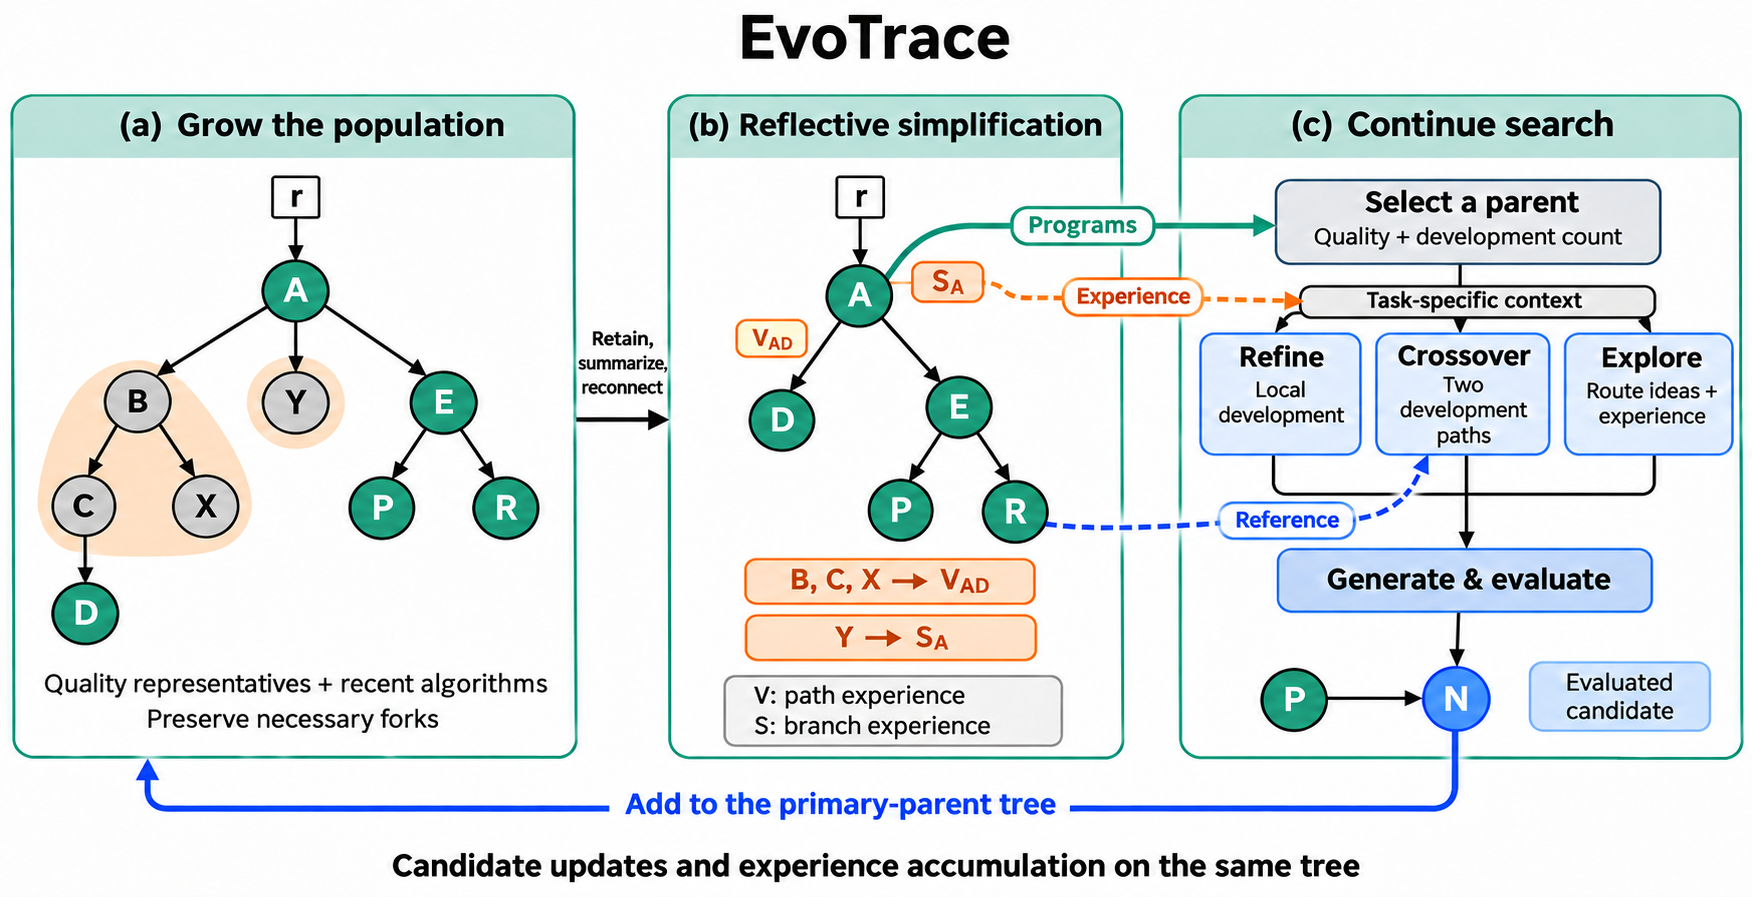
\includegraphics[keepaspectratio,alt={EvoTrace整体框架。 保留集合决定种群怎样简化，以及移除经历在哪里凝练为经验。更新后的树提供可选程序与适合当前设计任务的经验。每次尝试选择一种算子，受评候选随后接入主父代树。虚线表示经验与交叉参考等信息输入。}]{figures/framework.png}}
\caption{EvoTrace整体框架。
保留集合决定种群怎样简化，以及移除经历在哪里凝练为经验。更新后的树提供可选程序与适合当前设计任务的经验。每次尝试选择一种算子，受评候选随后接入主父代树。虚线表示经验与交叉参考等信息输入。}
\end{figure}

\subsubsection{3.2. 树状种群}\label{ux6811ux72b6ux79cdux7fa4}

记当前树为\(T=(\mathcal N\cup\{r\},\mathcal E)\)，其中\(r\)是不包含实现的虚拟根。算法节点保存代码、计算过程描述、适应度\(f(v)\)或失败反馈，以及实际使用记录。每个节点只有一个主父代。Crossover另存参考算法来源，该来源不增加第二条结构边。全部保留的可行节点都可继续开发，内部节点与叶节点使用相同资格。

树保存两类经验。节点上的\textbf{选择经验}（selection
experience）\(S_v\)凝练归属该位置的已移除旁支；边上的\textbf{变异经验}（variation
experience）\(V_{uv}\)凝练保留端点之间被收缩的发展过程及中间节点的同轮移除旁支。两个名称对应产生摘要的简化操作。两类经验都可描述改进、同分、退步或失败，收缩路径也可包含净退步。选择经验进入生成上下文与后续反思，父代采样则使用适应度和开发次数。虚拟根可以承接退出显式种群的初始路线经验。普通边表示一次生成尝试，收缩边明确标为一个发展阶段。

初始化与Explore开启开发路线，Refine与Crossover继承主父代路线。路线按实现的Init/Explore起点分组。原始入口被移除后，后代仍保存路线编号。路线用于父代分配和局部上下文组织。Explore入口可以收缩；两端路线不同的重连边保留Explore类型。

\subsubsection{3.3.
动态反思简化}\label{ux52a8ux6001ux53cdux601dux7b80ux5316}

初始化完成后，每次有受评实现入树，系统执行三个步骤：选择算法、保留必要分叉、划分移除区域。三个步骤均基于同一份简化前快照。

\textbf{选择质量代表。}
设\(\mathcal P\subseteq\mathcal N\)是可行节点集合，按适应度和生成先后排序。节点的秩质量为

\[
q(v)=1-\frac{\operatorname{rank}(v)}{\max(1,|\mathcal P|-1)},
\qquad v\in\mathcal P,
\tag{1}
\]

最优节点的排名为0。系统必留冠军，再按排名检查\(q(v)\geq0.50\)的候选。仅当同路线后代的适应度严格更好时，候选被标为已超越，不进入质量代表集合。该候选仍可因近期使用或必要分叉保留；若被移除，其经历按最终保留集合确定的区域交接。若候选与已有质量代表的标准化源码相同，或抽象语法树（abstract
syntax tree,
AST）距离小于\(0.08\)，则视为已被覆盖。两者适应度相差不超过\(10^{-9}\)时，距离门槛为\(0.20\)。未被覆盖的候选进入质量代表集合\(\mathcal R\)。参与覆盖判断的已有代表，其适应度不差于当前候选。

结构距离是AST父子类型特征与遍历二元组的多重集Jaccard距离。特征保留运算类型、被调用函数名和控制结构，普通变量身份及数值取值不作为取值特征。标准化源码相同是独立判据，保留变量与常数，只忽略排版、注释和文档字符串。两种判据共同构成实现中的覆盖启发式。

\textbf{保留近期使用算法。}
评价时钟\(t\)按实际程序评价推进。可行节点的最近使用时刻\(u(v)\)在出生时刷新；作为Refine/Crossover主父代产生受评尝试时刷新。Explore和只读交叉参考均不刷新原节点时钟。记\(p(v)\)为\(v\)在树上的父代，近期集合为

\[
\mathcal U=\{v\in\mathcal P:t-\max(u(v),u(p(v)))<W\},
\qquad W=40,
\tag{2}
\]

其中父代为虚拟根或属于其他路线时只取\(u(v)\)。同路线尝试可以共同失去近期资格；质量代表与必要分叉仍保留。

失败执行与修复重评均推进时钟。仅在提示中展示节点，或为了结构连接而保留节点，不刷新时间。近期保留维持窗口内的开发资格，实际开发机会仍由父代采样决定。

\textbf{保留必要分叉。} 最终保留集合为

\[
\mathcal K=\{r\}\cup\mathcal R\cup\mathcal U
\cup\operatorname{LCA}(\mathcal R\cup\mathcal U),
\tag{3}
\]

其中，\(\operatorname{LCA}(A)\)表示\(A\)内节点两两最近共同祖先（lowest
common ancestor,
LCA）的集合，保留连接已选节点所需的分叉。未被选中且不承担这些分叉的中间祖先可以收缩。质量代表先选定，再加入近期节点和必要连接。因此，仅因近期性或连接职责而保留的节点，不会排斥更好的质量代表。一次更新只计算一次排名和代表集合。保留规模由最近使用、质量差异与分叉结构共同形成，规则不设固定容量。

\textbf{联合划分路径与旁支。}
对每个保留算法，在原树上寻找最近保留祖先，两者之间被移除的中间节点组成路径收缩区域。其余移除节点向上寻找首个不属于旁支移除集合的祖先：若它是被收缩中间节点，旁支并入该路径区域；若是保留节点或虚拟根，则由其承接旁支区域。每个移除节点在本轮维护中只属于一个区域，同一承接位置的多条旁支合并处理。

同次更新可以缩短路径并剪除其旁支。例如，原树为\(A\rightarrow B\rightarrow C\rightarrow D\)，另有\(B\rightarrow X\)和\(A\rightarrow Y\)，只保留\(A,D\)时，\(B,C\)进入收缩路径，\(X\)也进入该路径区域，共同凝练到\(V_{AD}\)；旁支\(Y\)更新\(A\)处的\(S_A\)。早先已附着于\(B,C\)的经验随原承载节点进入路径区域。

\begin{figure}
\centering
\pandocbounded{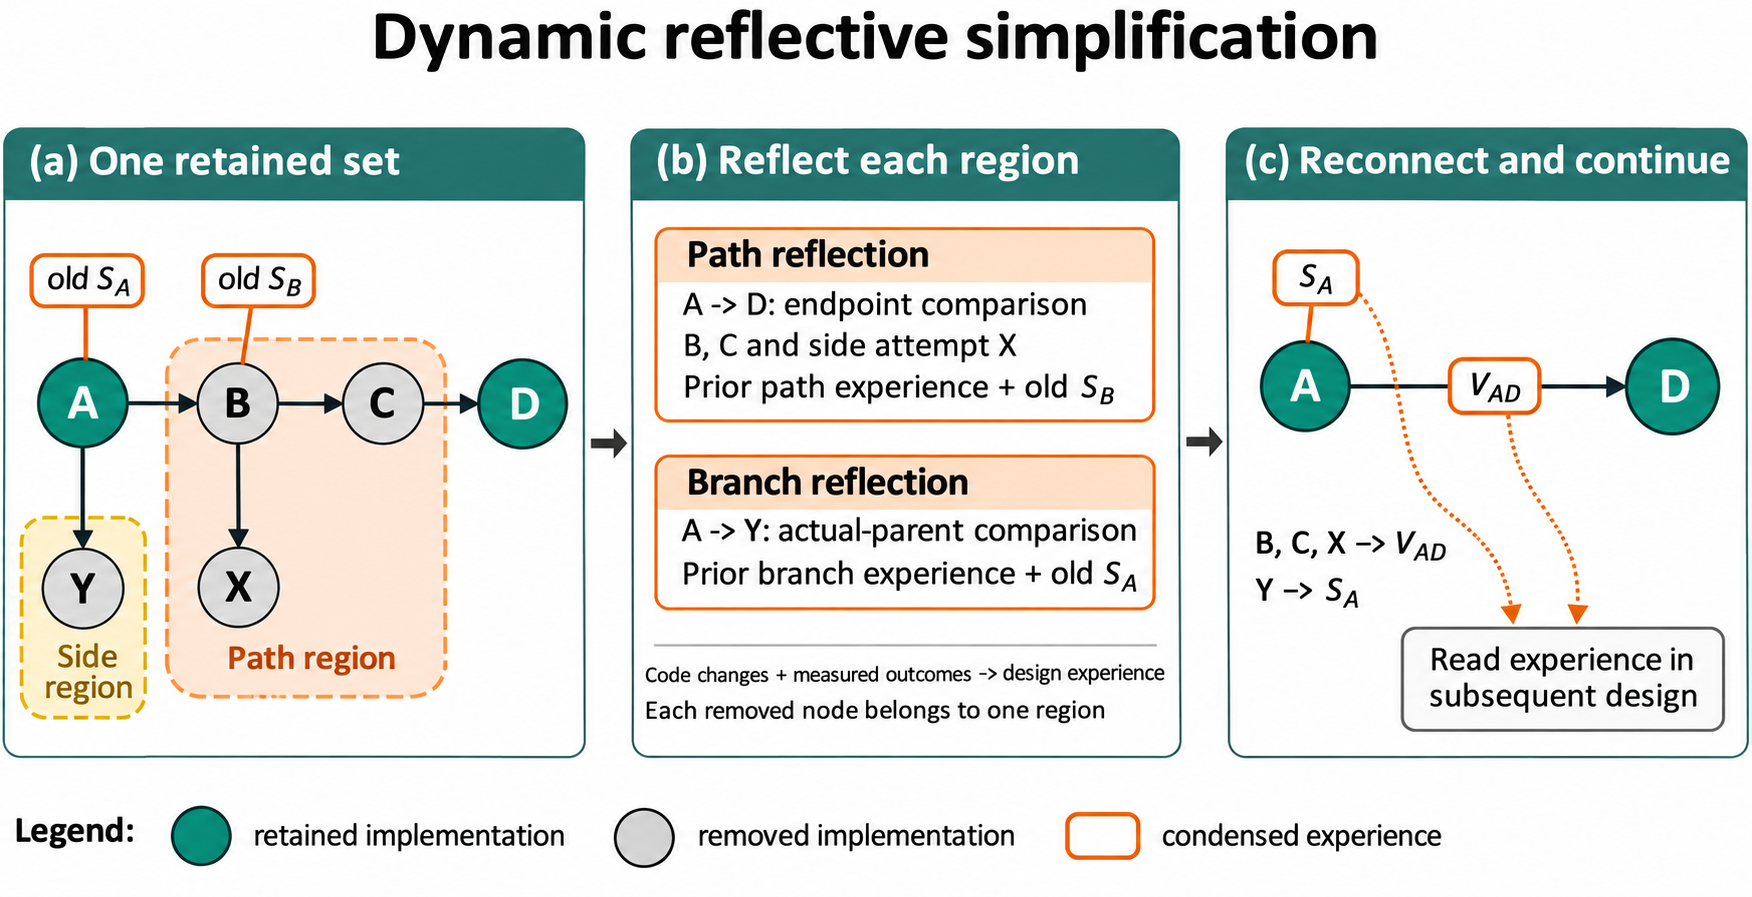
\includegraphics[keepaspectratio,alt={经验随保留结构交接。 保留A和D时，中间版本B、C及旁支X组成同一路径区域，凝练为重连边上的V\_\{AD\}；另一旁支Y更新S\_A。旧经验随承载位置交接：原S\_B进入路径摘要，原S\_A与Y的经历合并。}]{figures/reflective-simplification.png}}
\caption{经验随保留结构交接。
保留A和D时，中间版本B、C及旁支X组成同一路径区域，凝练为重连边上的\(V_{AD}\)；另一旁支Y更新\(S_A\)。旧经验随承载位置交接：原\(S_B\)进入路径摘要，原\(S_A\)与Y的经历合并。}
\end{figure}

\subsubsection{3.4. 区域反思}\label{ux533aux57dfux53cdux601d}

\textbf{按区域反思。}
每个最终路径区域与每组旁支区域各调用一次反思。路径反思读取保留端点代码、端点净差分、中间受评实现及其结果、同轮移除旁支，以及区域内已有的节点和边经验。旁支反思读取承接位置的实现（若存在）、移除尝试相对各自真实父代的差分、评价或错误反馈，以及相关旧经验。虚拟根没有算法实现时，以任务级起点提供上下文。已经收缩的输入明确作为发展阶段展示。旁支比较使用每次尝试的实际父代。当前比较以程序计算的结果标签提供给反思模型；原始分数保留在日志，路径经验的端点分数由程序附加。两类反思均区分Explore初稿与局部修改，将每次观察结果归于具体受评实现。

反思提示要求简洁描述所尝试的计算及其观察结果，并在证据支持时给出可能解释。提示区分整段起终点的净变化与中间比较，将共同修改的部件作为组合改动处理。提示要求模型保留与当前测量比较一致的旧经验；比较标签本身由程序计算。生成时的设计理由不进入证据。同次更新中的各区域读取同一原始快照，本轮新摘要不在同轮再次使用。

路径反思更新重连边上的\(V_{uv}\)。旁支反思更新承接位置的\(S_u\)，并吸收该位置原有的选择经验。后续更新若移除经验载体，累计经验继续归入新的对应区域。该递归过程使中间实现退出显式种群后，发展过程仍有凝练表示。树中摘要与保留实现共同提供发展上下文，尝试档案保存完整原始证据。

\subsubsection{3.5.
从维护后的树继续搜索}\label{ux4eceux7ef4ux62a4ux540eux7684ux6811ux7ee7ux7eedux641cux7d22}

\textbf{父代与参考选择。}
EvoTrace适配ShinkaEvolve的加权父代采样\citep{shinka}。记\(D(v)\)为节点\(v\)按原始Init/Explore路线编号归属的路线；每条非空路线只包含当前保留可行节点。定义

\[
w(v)=\sigma\!\left(10\frac{m-f(v)}{s}\right)\frac{1}{1+c(v)},
\tag{4}
\]

\[
P(D)\propto\max_{u\in D}w(u),\qquad P(v\mid D)=\frac{w(v)}{\sum_{u\in D}w(u)},
\tag{5}
\]

其中，\(\sigma\)为sigmoid函数，\(c(v)\)为使用\(v\)作为主父代的受评Refine/Crossover尝试数。每次采样前在当前树上重算质量代表，以其适应度中位数\(m\)及中位数绝对偏差尺度\(s\)进行归一化。全部保留可行节点均可参与采样，概率为\(P(D(v))P(v\mid D(v))\)。固定权重时，加入一个不超过所属路线最大权重的版本，不改变路线概率。实际更新仍可通过新的最大值、父代进一步开发或代表集合及其归一化的变化，改变路线概率。

选定主父代后，系统以\(0.45\)、\(0.25\)、\(0.30\)的概率分别选择Refine、Crossover和Explore。Crossover先排除主父代和标准化源码重复项，再在实际可用参考中计算秩质量，保留不低于\(0.30\)的候选。系统优先考虑尚未使用的有序``主父代---参考''配对，并在其中选择AST距离最大者；同距离时依次取适应度较好、生成较早者。合格配对全部使用过后允许复用；没有合格参考时执行Refine。

\textbf{按设计任务组织上下文。} 三个算子读取同一种群的不同视图：

{\def\LTcaptype{none} % do not increment counter
\begin{longtable}[]{@{}
  >{\raggedright\arraybackslash}p{(\linewidth - 4\tabcolsep) * \real{0.3333}}
  >{\raggedright\arraybackslash}p{(\linewidth - 4\tabcolsep) * \real{0.3333}}
  >{\raggedright\arraybackslash}p{(\linewidth - 4\tabcolsep) * \real{0.3333}}@{}}
\toprule\noalign{}
\begin{minipage}[b]{\linewidth}\raggedright
算子
\end{minipage} & \begin{minipage}[b]{\linewidth}\raggedright
结构上下文
\end{minipage} & \begin{minipage}[b]{\linewidth}\raggedright
当前设计任务
\end{minipage} \\
\midrule\noalign{}
\endhead
\bottomrule\noalign{}
\endlastfoot
Refine &
当前代码与成绩；本路线形成路径及直接来源摘要；节点选择经验；可见出边尝试或发展阶段
& 结合形成过程和已评价替代尝试修改当前计算 \\
Crossover &
两份实现；同路线的共同祖先与双支，或跨路线各自的局部发展与来源摘要；相关节点和边经验；主父代的可见子尝试
& 决定迁移哪些计算以及怎样融合 \\
Explore &
不同路线的入口思想；所选路线中生成次序最新的保留版本；节点、边和根经验；一份已有实现
& 构造主要计算方式不同的替代算法 \\
\end{longtable}
}

普通转移展示相对真实父代的差分和结果，收缩转移展示端点结果和累计变异经验。差分序列提供解释变化所需的基准代码。同路线Crossover只展示一次共同祖先；跨路线时简述历史来源，不展开旧路线。Explore不在每段经验前重复完整设计描述。Explore先组织思想与经验，再给出一份现有实现，使模型可以重新考虑表示或计算过程。

上下文构造先组织相关保留材料。若生成提示超过输入预算，系统依据实际释放的token数量，减少完整路径条目、尝试条目或路线条目。当前源码、参考源码及解释差分所需的基准保持可用。输入适配只改变单次提示视图，不改变树、保留决策或经验归属。每个算子返回完整实现及其计算过程描述。

\subsubsection{3.6. 搜索过程}\label{ux641cux7d22ux8fc7ux7a0b}

算法1给出完整过程。初始化在同一预算内获得五个可行程序。每次生成尝试最多允许一次修复，并最多贡献一个最终受评节点。修复重评另计评价预算。没有产生程序评价的尝试不入树，也不推进评价时钟。

\par\noindent\begin{minipage}{\linewidth}
\begin{verbatim}
算法1：EvoTrace
输入：任务接口、评价器、大语言模型、评价预算B
建立虚拟根、空种群与尝试档案
当评价预算未耗尽且未满足停止条件时：
    若可行初始程序少于五个：
        构造初始化提示
    否则：
        采样父代与算子；需要时选择参考
        构造并适配对应的树上下文视图
    生成并评价程序，最多允许一次修复
    记录全部模型请求与评价结果
    若本次存在受评程序：
        接入最终受评版本；更新实际使用记录
        若初始化完成：
            在同一快照上选择质量代表与近期节点
            补入必要分叉祖先，确定最终保留集合
            在该快照上划分移除路径与旁支
            逐区域反思
            重连保留节点并附着对应经验
    提交本次尝试与对应种群更新
返回完整档案中搜索适应度最好的可行程序
\end{verbatim}
\end{minipage}


每次更新保留当前最佳算法，并将每个保留节点重连到其最近保留祖先。两两分叉闭包使收缩路径互不重叠，其余移除节点各有唯一承接区域。附录B给出这些结构性质的论证。

\subsection{4. 初步实验}\label{ux521dux6b65ux5b9eux9a8c}

我们在四个组合优化任务上检查实现，并报告一次冻结的早期搜索快照。快照来自2026年11月14日冻结源码的运行批次，包含每任务种子0、1、2，共12路独立搜索。每路目标预算为1000次评价。快照时各路已完成62--97次评价。我们在共同的60次评价位置报告训练分数，并分析各路已提交前缀中的种群更新。独立测试与完整搜索比较需要使用完成后的运行结果。

\subsubsection{4.1.
任务与评价条件}\label{ux4efbux52a1ux4e0eux8bc4ux4ef7ux6761ux4ef6}

每个任务在固定求解器内演化一个函数。TSP演化逐步构造中的下一节点选择；CVRP与OP演化蚁群算法的边先验；FSSP演化引导式局部搜索使用的矩阵与作业选择计算。目标依次为平均回路长度、平均路线长度、平均最大完工时间与负的平均收集奖励，均采用最小化约定。

每任务使用16个训练实例。50个不重叠的同规模实例用于最终所选程序的测试。一次完整训练评价共享160秒时限，评价进程内存上限为2
GiB，使用一个工作进程。失败消耗评价预算，修复重评单独计数。模型池提供关闭原生思考的Qwen3.8-27B。生成温度为1.0，输出上限16384词元；反思温度为0.3，输出上限1536词元。其余任务与采样设置见附录D。

搜索结束后先固定训练成绩最好的有效程序，再执行测试。测试结果不参与选择。模型请求及返回的词元用量与程序评价分别记账，从而区分经历压缩的模型成本和搜索评价预算。

\subsubsection{4.2.
共同预算下的训练分数}\label{ux5171ux540cux9884ux7b97ux4e0bux7684ux8badux7ec3ux5206ux6570}

表1报告60次评价后的训练最优分数。标准差为三路独立搜索之间的样本标准差。各任务保留原始计量单位；OP最小化负奖励，因此越负越好。

\Needspace{12\baselineskip}
\begin{longtable}[]{@{}lrrr@{}}
\caption{60次评价后的训练最优值，越小越好。}\tabularnewline
\toprule\noalign{}
任务 & 种子0 / 1 / 2 & 均值 & 标准差 \\
\midrule\noalign{}
\endfirsthead
\toprule\noalign{}
任务 & 种子0 / 1 / 2 & 均值 & 标准差 \\
\midrule\noalign{}
\endhead
\bottomrule\noalign{}
\endlastfoot
TSP & 5.8774 / 5.9590 / 5.9229 & 5.9198 & 0.0409 \\
CVRP & 8.5584 / 8.6008 / 8.7791 & 8.6461 & 0.1171 \\
FSSP & 3880.31 / 3879.12 / 3892.25 & 3883.90 & 7.26 \\
OP & -14.2787 / -14.5994 / -14.2663 & -14.3815 & 0.1888 \\
\end{longtable}

\begin{figure}
\centering
\pandocbounded{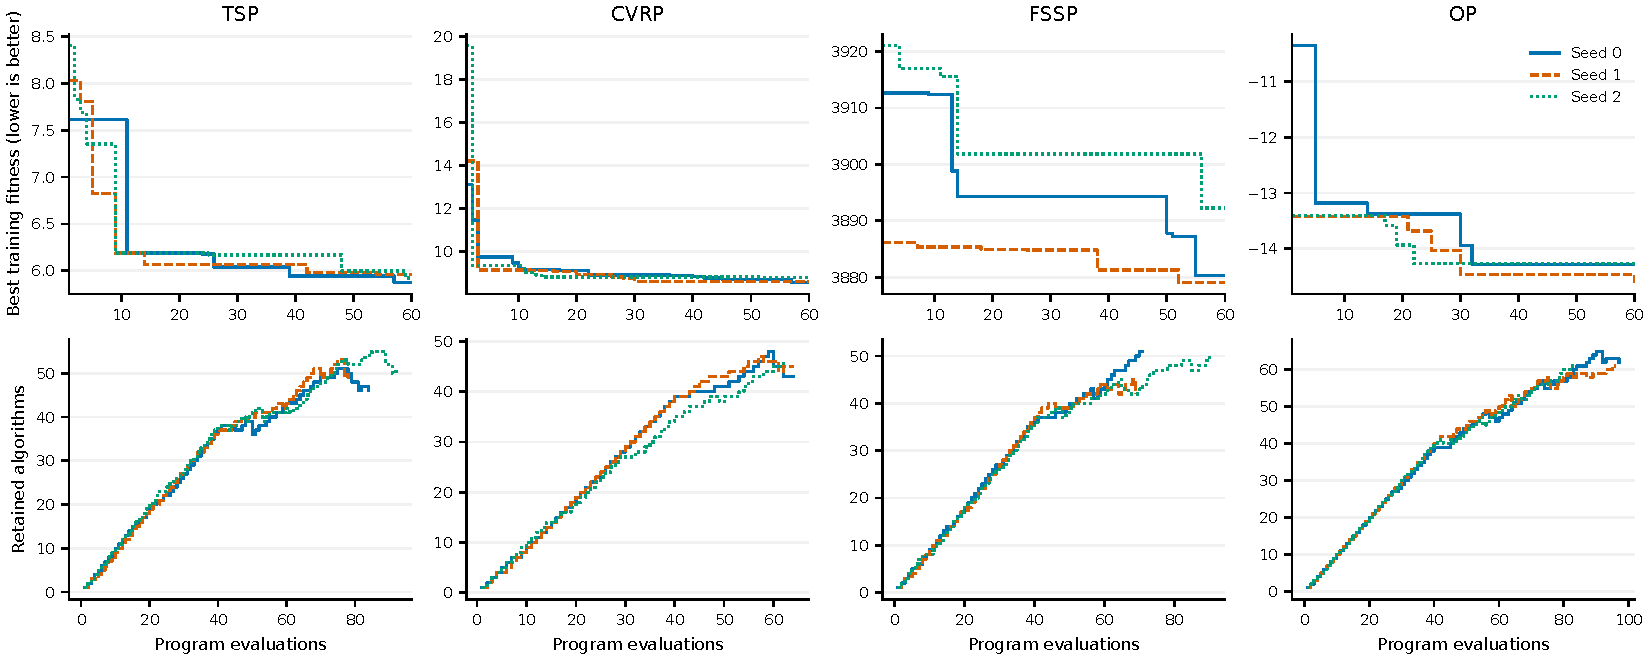
\includegraphics[keepaspectratio,alt={冻结运行中的早期搜索。 上排展示各任务三路搜索前60次评价的训练最优分数，采用共同可观察范围。下排按每次已提交受评入树及其对应移除重建保留算法数，延伸至各路观察终点，并与已保存的完整树快照核对。细线分别表示三个种子。这些轨迹描述当前阶段的搜索与种群维护过程。}]{figures/early-search.pdf}}
\caption{冻结运行中的早期搜索。
上排展示各任务三路搜索前60次评价的训练最优分数，采用共同可观察范围。下排按每次已提交受评入树及其对应移除重建保留算法数，延伸至各路观察终点，并与已保存的完整树快照核对。细线分别表示三个种子。这些轨迹描述当前阶段的搜索与种群维护过程。}
\end{figure}

\subsubsection{4.3.
种群如何压缩历史}\label{ux79cdux7fa4ux5982ux4f55ux538bux7f29ux5386ux53f2}

冻结前缀包含951次评价和894次已提交生成尝试。其中207次更新发生结构简化，将286个移除实现分配到47个路径区域和175个旁支区域。对已记录计划的核对确认，每个移除节点在相应更新中恰好归属一个区域。快照时各路保留42--62个算法；12路共接入894个节点，其中608个仍为显式节点。相对62--97次评价的前缀，40次评价的近期窗口占据相当大的范围。已记录区域以旁支为主（222个中175个），因此早期简化主要体现为旁支凝练。

222个区域产生222次模型反思，本快照没有回退摘要。186个区域只包含一个本轮移除实现，最大区域包含五个。因此，压缩经常以增量方式进行：一次新的移除可以与载体上已积累的经验共同进入反思。本轮移除节点数描述当前更新，不等于摘要所代表的全部历史规模。

反思调用累计报告505171个输入词元与29283个输出词元。输入包括任务说明、端点代码、比较和继承经验，因此这两个数表示模型调用成本，其比值不衡量语义保留程度。这些记录确认了显式实现向节点和边经验的结构交接。附录E计划的固定状态对照将固定树快照、父代、算子和参考，只改变相同移除区域的表示方式，以检验经验对后续生成的作用。

\subsection{5. 讨论}\label{ux8ba8ux8bba}

\textbf{种群作为经历的表示。}
EvoTrace共同维护两种历史形式。保留程序可继续执行和开发；移除区域通过带有发展关系的摘要继续存在。后续更新再次改变这种表示，将旧经验交给新的节点或边。候选维护因而同时组织后续生成可以利用的经历。

\textbf{增量压缩与保真度。}
区域规模表明，反思压缩经常通过连续的小规模更新累积，这使多轮交接中的摘要保真度成为重要变量。提示保留明确的比较结果、实际父代关系及观察与解释的区别，档案提供核对这些陈述所需的代码和评价。组合修改的解释对应被评价的整组变化；将结果归因于其中一个部件，需要额外比较。

\textbf{研究范围。}
当前证据覆盖同一模型家族在四任务上的早期搜索，确认了结构简化与经验交接的运行过程。最终独立测试和受控历史读取对照将检验算法质量及压缩的作用。

\subsection{6. 结论}\label{ux7ed3ux8bba}

EvoTrace将候选竞争与设计经验积累联系起来。其出发点是区分实现的继续开发价值与经历的后续参考价值。树状种群使这一区分落实为算法：一次保留决策共同确定显式候选、压缩区域及经验承接位置。动态反思简化随种群变化继续交接摘要，算子视图将相关经验送入后续生成。由此，搜索状态同时保存可执行算法及其发展过程的凝练表示。

\subsection{附录A.
默认设置}\label{ux9644ux5f55a.-ux9ed8ux8ba4ux8bbeux7f6e}

{\def\LTcaptype{none} % do not increment counter
\begin{longtable}[]{@{}
  >{\raggedright\arraybackslash}p{(\linewidth - 2\tabcolsep) * \real{0.5000}}
  >{\raggedright\arraybackslash}p{(\linewidth - 2\tabcolsep) * \real{0.5000}}@{}}
\toprule\noalign{}
\begin{minipage}[b]{\linewidth}\raggedright
组成
\end{minipage} & \begin{minipage}[b]{\linewidth}\raggedright
设置
\end{minipage} \\
\midrule\noalign{}
\endhead
\bottomrule\noalign{}
\endlastfoot
初始化与评价预算 & 五个可行初始程序；1,000次实际程序评价 \\
近期保留 & 自身或同路线树上父代距出生或局部开发少于40次评价 \\
质量代表 &
秩质量不低于0.50，由优到劣检查；排除被同路线严格更优后代超越或已被覆盖的候选 \\
覆盖距离 & 小于0.08；适应度相差不超过\(10^{-9}\)时小于0.20 \\
父代采样 &
sigmoid系数10；按自身同路线开发次数折扣；路线最大权重与路线内归一化 \\
算子先验 & Refine 0.45；Crossover 0.25；Explore 0.30 \\
参考资格 & 排除主父代与相同标准化源码后，秩质量不低于0.30 \\
路线视图筛选 &
入口标准化源码不同且AST距离不低于0.12；按最新保留版本次序组织 \\
演化生成输入 & 30,000 tokens，必要时按完整条目缩减 \\
生成模型 & 温度1.0，输出上限16,384 tokens \\
反思模型 & 温度0.3，输出上限1,536 tokens；约120词的段落，证据少时更短 \\
\end{longtable}
}

式（4）的尺度\(s\)为中位数绝对偏差（median absolute deviation,
MAD），下限\(10^{-6}\)。MAD不超过\(10^{-9}\)时，使用大于\(10^{-9}\)的非零绝对偏差中位数，并保留同一下限。无非零偏差时使用尺度下限。实现以对数权重完成两级归一化；下溢的最终概率用最小正浮点值表示。参考池只有一个候选时，其秩质量为1。

输入长度优先使用服务tokenizer计数。没有tokenizer的独立客户端以UTF-8字节数作为保守代理，并记录计数方式。输入适配用于三类演化生成提示；必要材料仍超窗时明确报错。

反思调用或解析失败时，系统使用960字符预算的确定性摘要，继续完成结构更新。完整区域输入和模型响应仍保存在档案中。连续十次尝试没有程序评价时，搜索提前停止。种群更新与产生它的尝试共同提交，恢复读取已提交更新，不重复调用对应反思。

\(c(v)\)统计以\(v\)为主父代的受评Refine/Crossover尝试，包括失败及后来被移除的尝试。同次尝试中的修复、Explore、只读参考、结构重连及继承历史不增加该计数。

\subsection{附录 B.
单次更新的结构性质}\label{ux9644ux5f55-b.-ux5355ux6b21ux66f4ux65b0ux7684ux7ed3ux6784ux6027ux8d28}

设有限有根树中的保留集合\(K\)包含虚拟根、主动保留节点及这些节点两两之间的最近共同祖先。将每个非根保留节点重连到其最近保留祖先。

\textbf{连通性与无环性。}
每个保留节点的祖先链按祖先关系全序排列，且包含虚拟根，因此最近保留祖先唯一。每条重连边严格沿原祖先链向上。持续沿边上行必然到达根，不能形成环，所得结构仍为\(K\)上的有根树。

\textbf{收缩路径互不重叠。}
假设一个移除节点同时位于两条保留端点连接的内部。若两个后代端点在其下方分叉，其最近共同祖先位于重叠处且必须属于\(K\)，与连接内部全部移除矛盾；若一个端点是另一个的祖先，前一个保留端点会截断后一条连接。因此，每个移除中间节点只属于一条收缩路径。

\textbf{区域归属唯一。}
从全部移除节点中去掉收缩路径内部节点。其余每个节点沿祖先链向上，有唯一的首个不属于该剩余集合的祖先。这个祖先或者是路径中间节点，或者是保留节点，包括根。前者使该节点进入唯一的路径区域，后者使其进入该祖先的旁支区域。因此，每个移除节点在本轮更新中恰好被分配一次。该性质针对移除实现的归属；保留端点代码可以作为比较背景出现在多个反思输入中。

\textbf{最优候选保留。}
代表选择首先纳入当前最佳可行节点，且不会再从代表集合移除它，因此它属于\(K\)。这项性质描述当前种群；尝试档案独立保存最终选择所需的最佳可行程序。

以上性质描述结构及分配。语言摘要的具体内容由反思模型及输入证据决定。

\subsection{附录 C.
反思提示模板}\label{ux9644ux5f55-c.-ux53cdux601dux63d0ux793aux6a21ux677f}

两类反思均先提供任务、接口和目标方向，再列出实现、代码差分、程序计算的结果标签、错误以及旧经验。英文稿附录C逐字收录实际任务与输出模板。核心要求如下。

\textbf{路径反思。}
先陈述保留起点到终点的净结果，并共同描述计算变化。中间步骤和旁支只在提供额外信息时纳入，保留各自比较对象及结果标签。解释以``一种可能的解释是''引出，并限定于被测实现。Explore表示新计算方向的初稿，其结果不代表整个方向的潜力。组合变化不能单独确定部件贡献。输出一个含\texttt{experience}字符串的JSON对象，通常不超过120个英文词。

\textbf{旁支反思。}
每个尝试仅与其实际父代比较；无算法父代的初始实现不具有父代相对改进。先说明起始计算、整组修改及观察结果，再按证据给出可能解释。旧经验只有在比较对象与条件清楚时才继续保留。输出格式和长度约束与路径反思相同。

两类模板都要求以当前程序计算的比较为准，区分整段净变化与中间变化，避免从同分推导程序等价，也不将经验写成未来设计指令。模板原文保存在\texttt{evotrace\_v2/reflection.py}。

\subsection{附录 D.
复现与记账}\label{ux9644ux5f55-d.-ux590dux73b0ux4e0eux8bb0ux8d26}

当前部署在启动前冻结方法源码、任务定义、评价器和采样配置。每条已提交尝试记录生成程序、含修复在内的全部评价、父代与参考编号、上下文视图及种群更新。更新记录包括移除区域、反思响应和结果树。恢复重放已提交更新，不重复请求反思。一次尝试的最终受评版本进入在线树，修复前版本保存在尝试档案中。

搜索种子为0、1、2。TSP训练使用50节点欧氏实例，数据种子2024。CVRP使用30只蚂蚁、100轮ACO迭代；OP使用20只蚂蚁、50轮迭代；两项ACO任务的求解器种子均为1234。训练评价种子为730241。冻结任务配置完整规定FSSP实例与求解器设置。生成提示提供接口与目标；实例数量、数据划分和求解器迭代次数属于评价条件。

生成采样另设top-p为0.8、top-k为20、presence
penalty为1.5。公共模型池在多个端点间分配调用，返回的模型名包括\texttt{Qwen3.8-27B}和\texttt{qwen3.8-27b-awq}。端点名称本身不能证明数值推理完全一致。每次调用的元数据记录端点及返回用量。服务接口故障与候选执行失败分别记账。

交付的证据快照保存每路来源路径、已提交尝试文件的SHA-256、捕获时间、不含凭据的配置及第4节使用的精确评价前缀。分数表和图3由快照生成。更新快照需要显式执行；重新编译论文不会刷新实验数据。

\subsection{附录 E.
核心主张的评价设计}\label{ux9644ux5f55-e.-ux6838ux5fc3ux4e3bux5f20ux7684ux8bc4ux4ef7ux8bbeux8ba1}

以下方案规定后续检验，第4节报告的是已观察到的部署快照。

\textbf{完整搜索。}
冻结各比较方法后，每任务运行三个搜索种子。对齐任务接口、数据、候选评价限制、生成设置、评价记账和最终选择。原方法若按生成而非评价计数，单独记录其预算定义。报告训练轨迹、按训练选定程序的测试分数、逐种子值、失败，以及生成、修复和反思成本。

\textbf{固定状态的历史表示。}
从预先指定的评价位置抽取状态，不按后续成功挑选。固定父代、算子、参考、当前代码及任务说明，比较省略历史、相同区域原始材料及实际反思摘要。每条件重复采样，以快照为配对单位，同一快照生成的多个后代不作为独立搜索路次。按任务及算子报告分数、执行成功、父代相对改进及输入词元；超过窗口的原始历史单列。

\textbf{经验位置。}
固定所选摘要与输入预算，比较原有结构组织和保留来源标签的共享列表，区分结构分组与文本可用性各自的作用。

\textbf{摘要保真度。}
按任务、区域类型与既往交接次数记录随机抽样。比较方向与评价档案核对，计算描述与实际代码核对，分别记录结果、代码描述和解释的错误。后续提示是否读到经验单独追踪，不直接等同于经验造成改进。

\bibliography{references.bib}

\end{document}
